\documentclass[11pt]{article}

\usepackage[margin=1in]{geometry}
\usepackage[T1]{fontenc}
\usepackage[utf8]{inputenc}
\usepackage{lmodern}
\usepackage{graphicx}
\usepackage{amsmath,amssymb,amsfonts}
\usepackage{textcomp}
\usepackage{xcolor}
\usepackage[hidelinks]{hyperref}
\usepackage{booktabs}
\usepackage{tikz}
\usetikzlibrary{positioning, arrows.meta, fit}

\hyphenation{nano-chat permu-tational dual-stream}

\setlength{\parskip}{2pt}
\setlength{\textfloatsep}{6pt plus 2pt minus 2pt}
\setlength{\intextsep}{6pt plus 2pt minus 2pt}

\begin{document}

\title{\Large\textbf{Dual-stream LUT transformer: a short report on \texttt{exp303}}\vspace{-4pt}}
\author{Anatoly Starostin}
\date{}
\maketitle
\vspace{-18pt}

\noindent\textbf{Scope.}
A one-experiment delta to the May 2026 status report.
\texttt{exp303} is the current head of a new architectural branch --- the \emph{dual-stream} variant of the LUT transformer.
We assume the reader has the May report at hand for the LUT primitive (\texttt{TinyMultiHeadLut}), the V2D / D2V layers, and the single-stream baseline (\texttt{exp265}) that this branch is being measured against.

% ======================================================================
\section{The dual-stream variant}
\label{sec:arch}

The May-report model is what we now call the \emph{single-stream} architecture: each block reads and writes the same ranking embedding $\mathbf{x}_\ell \in \mathbb{R}^{B \times T \times E}$ at $E = 96$, the inter-block signal is rank-canonicalised by V2D / D2V at every block boundary, and per-layer outputs are concatenated and pushed through a wide MLP unembedder to vocabulary logits.
That MLP unembedder dominates the model's per-token weight bandwidth (May report, Sec.\ ``Bandwidth'').

The dual-stream variant adds a second carrier alongside the ranking embedding:
\begin{itemize}
\setlength{\itemsep}{1pt}
    \item $\mathbf{x}^{\text{lut}}_\ell \in \mathbb{R}^{E}$, $E = 64$ --- the LUT carry between blocks.
    \item $\mathbf{x}^{\text{resid}}_\ell \in \mathbb{R}^{D}$, $D = 384$ --- a vanilla-baseline-width real-valued residual stream that every block writes into via a per-block \texttt{residual\_lut} ($\mathbb{R}^E \to \mathbb{R}^D$).
\end{itemize}
The unembedder is then a plain untied linear $\mathbb{R}^D \to \mathbb{R}^V$ on the final residual stream, in place of the wide concat-MLP.
There is no V2D / D2V at the block boundary --- the LUT carry is the LayerNorm'd raw out-projection output, with no rank canonicalisation enforced on the block-to-block signal.
The block layout is sketched in Figure~\ref{fig:block}.

\begin{figure}[!ht]
\centering
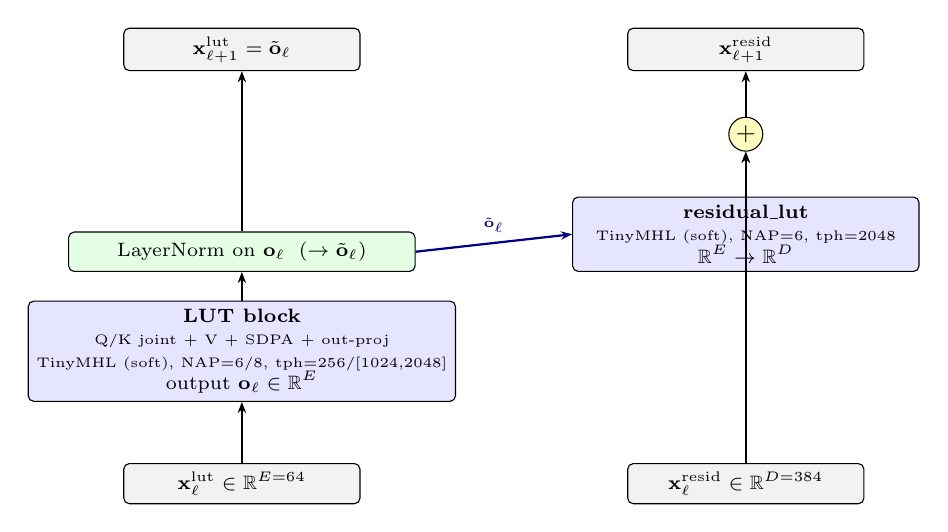
\begin{tikzpicture}[
    x=1cm, y=1cm,
    every node/.style={font=\scriptsize},
    box/.style={rectangle, draw, rounded corners=2pt, align=center, inner sep=3pt, fill=#1, minimum height=0.5cm},
    box/.default=blue!8,
    lut/.style={box=blue!10},
    ln/.style={box=green!10},
    add/.style={circle, draw, inner sep=1pt, fill=yellow!25, font=\small},
    arr/.style={-{Stealth[length=4pt]}, thick},
    sidearr/.style={-{Stealth[length=4pt]}, thick, blue!50!black},
]
    \node[box=gray!10, minimum width=3cm, anchor=south] (xlin)  at (-3.2, 0)   {$\mathbf{x}^{\text{lut}}_\ell \in \mathbb{R}^{E=64}$};
    \node[box=gray!10, minimum width=3cm, anchor=south] (xrin) at ( 3.2, 0)   {$\mathbf{x}^{\text{resid}}_\ell \in \mathbb{R}^{D=384}$};

    \node[lut, minimum width=4.4cm, anchor=south] (blk) at (-3.2, 1.3)
        {\textbf{LUT block}\\
         \tiny Q/K joint $+$ V $+$ SDPA $+$ out-proj\\
         \tiny TinyMHL (soft), NAP=6/8, tph=256/[1024,2048]\\
         output $\mathbf{o}_\ell \in \mathbb{R}^E$};

    \node[ln, minimum width=4.4cm, anchor=south] (ln) at (-3.2, 2.95)
        {LayerNorm on $\mathbf{o}_\ell$ \;($\to \tilde{\mathbf{o}}_\ell$)};

    \node[lut, minimum width=4.4cm, anchor=south] (rlut) at ( 3.2, 2.95)
        {\textbf{residual\_lut}\\
         \tiny TinyMHL (soft), NAP=6, tph=2048\\
         $\mathbb{R}^E \to \mathbb{R}^D$};

    \node[add, anchor=center] (sum) at ( 3.2, 4.7) {$+$};

    \node[box=gray!10, minimum width=3cm, anchor=south] (xlout)  at (-3.2, 5.5) {$\mathbf{x}^{\text{lut}}_{\ell+1} = \tilde{\mathbf{o}}_\ell$};
    \node[box=gray!10, minimum width=3cm, anchor=south] (xrout) at ( 3.2, 5.5) {$\mathbf{x}^{\text{resid}}_{\ell+1}$};

    \draw[arr] (xlin.north)  -- (blk.south);
    \draw[arr] (blk.north)   -- (ln.south);
    \draw[arr] (ln.north)    -- (xlout.south);
    \draw[sidearr] (ln.east)  -- node[above, font=\tiny] {$\tilde{\mathbf{o}}_\ell$} (rlut.west);
    \draw[arr] (xrin.north)   -- (sum.south);
    \draw[arr] (rlut.north)   -- (sum.south);
    \draw[arr] (sum.north)    -- (xrout.south);
\end{tikzpicture}
\caption{One block of the dual-stream LUT transformer (\texttt{exp303}). The LUT block (collapsed) is identical to the May-report block minus its V2D / D2V tail; the new piece is the \texttt{residual\_lut} that taps the LayerNorm'd block output and writes a $D$-dim contribution into the residual stream. After the last block, $\mathbf{x}^{\text{resid}}$ is LayerNorm'd and projected by a single linear $\mathbb{R}^D \to \mathbb{R}^V$ --- the wide concat-MLP unembedder of the single-stream model is gone. There is no FFN, no per-block residual on the LUT stream, and no weight decay on LUT weights, the token embedding, or the positional embeddings.}
\label{fig:block}
\end{figure}

% ======================================================================
\section{The lineage that produced \texttt{exp303}}
\label{sec:why}

\texttt{exp303} is the current head of a single-knob sweep that started from \texttt{exp272}; the table below is the chain of changes between siblings:
\begin{center}\small
\begin{tabular}{lll}
\toprule
Run & Single-knob change vs.\ predecessor & Final val bpb \\
\midrule
\texttt{exp272} & first dual-stream port from \texttt{exp265}, $E = 96$ & 1.6836 \\
\texttt{exp291} & drop weight decay from LUT weights and embeddings & 1.6749 \\
\texttt{exp294} & enlarge \texttt{out\_proj.tph\_per\_layer} by $4\times$ & 1.6636 \\
\texttt{exp300} & switch \texttt{v\_lut} and \texttt{out\_proj} to soft backward & 1.6573 \\
\textbf{\texttt{exp303}} & double \texttt{residual\_lut.tph}: $1024 \to 2048$ (NAP=6) & \textbf{1.6509} \\
\bottomrule
\end{tabular}
\end{center}
The companion run \texttt{exp302} (\texttt{residual\_lut} NAP $6 \to 8$, \texttt{tph} $1024 \to 512$, matched entry budget $2048 \cdot 2^{6} = 512 \cdot 2^{8}$) trailed \texttt{exp300} by $\approx 0.005$ bpb, so the \texttt{exp303} win is specifically a \emph{wider, shallower} \texttt{residual\_lut}, not just a bigger one.

% ======================================================================
\section{Result, read transparently}
\label{sec:result}

\begin{figure}[!ht]
\centering
\begin{minipage}[t]{0.55\linewidth}
\vspace{0pt}
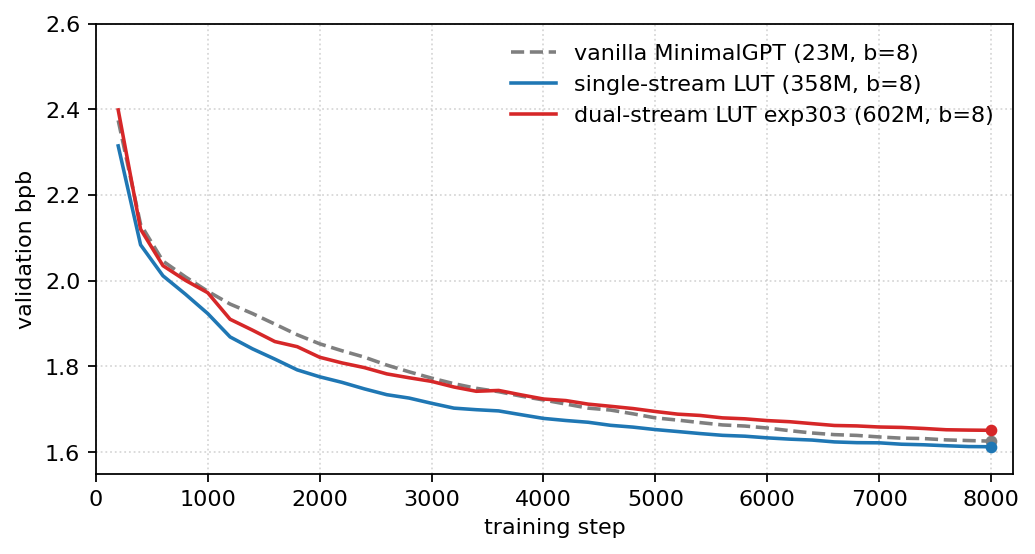
\includegraphics[width=\linewidth]{figs/exp303_val_bpb.png}
\end{minipage}\hfill
\begin{minipage}[t]{0.42\linewidth}
\vspace{0pt}\footnotesize
\setlength{\tabcolsep}{4pt}
\begin{tabular}{lrr}
\toprule
Run & Params & val bpb \\
\midrule
\texttt{exp001} (vanilla)            & 23 M  & 1.6256 \\
\texttt{exp265} (single-stream)      & 358 M & 1.6126 \\
\textbf{\texttt{exp303}} (dual)      & 602 M & \textbf{1.6509} \\
\midrule
\multicolumn{3}{l}{\emph{unmatched references:}} \\
\texttt{exp041} (vanilla, 48K)       & 23 M  & 1.3406 \\
\texttt{exp267} (single, $b{=}32$)   & 358 M & 1.4504 \\
\texttt{exp271} (vanilla, $b{=}32$)  & 23 M  & 1.3392 \\
\bottomrule
\end{tabular}
\end{minipage}
\caption{Validation bpb at 8K steps, $b{=}8$ (the matched comparison). Solid red: dual-stream LUT (\texttt{exp303}, 602M). Solid blue: single-stream LUT (\texttt{exp265}, 358M). Dashed grey: vanilla MinimalGPT (\texttt{exp001}, 23M). The lower group of the table lists the unmatched but informative reference points from the May report.}
\label{fig:val}
\end{figure}

\noindent\textbf{Within the dual-stream branch}, \texttt{exp303}'s 1.6509 is the new best by $\approx 0.03$ bpb over the next-best sibling (\texttt{exp300}).
\textbf{Across architectures at the matched 8K / $b{=}8$ budget}, however, it is \emph{worse} than the single-stream LUT \texttt{exp265} by $0.038$ bpb and \emph{worse} than vanilla MinimalGPT \texttt{exp001} by $0.025$ bpb.
The LUT carrier in this configuration costs $\approx 5\%$ relative bpb against the dense baseline while spending $26\times$ the parameters; vanilla and \texttt{exp303} are visually almost on top of each other in Figure~\ref{fig:val}, with vanilla finishing slightly ahead.
None of the larger comparators (lower group of the table) have been re-run in the dual-stream branch yet --- the $b{=}32$ batch lever (the single biggest contributor to the May report's headline numbers) has not been applied to \texttt{exp303}.

\noindent\textbf{What this is evidence for.}
A vanilla-width residual stream fed by per-block LUT taps is a \emph{viable} carrier --- it stays within $\approx 0.04$ bpb of the single-stream LUT model at the same compute, while replacing the dense MLP unembedder with a single linear layer.
The architectural change is large (no V2D / D2V at the block boundary, no concat-MLP unembedder, $E$ halved from 96 to 64), so this is a real positive datum.
The \texttt{residual\_tph} sweep also gave a clean small-signal answer: at fixed entry budget for \texttt{residual\_lut}, \emph{wider and shallower} (more tables, smaller NAP) beats deeper and narrower.

\noindent\textbf{What this is not evidence for.}
\texttt{exp303} does not beat the single-stream LUT branch on bpb at the matched 8K / $b{=}8$ budget, and does not beat vanilla.
The competitive comparisons against vanilla in the May report all came from the $b{=}32$ regime; the corresponding $b{=}32$ rerun of \texttt{exp303} has not been done yet.

% ======================================================================
\section{Next steps}
\label{sec:next}

\begin{enumerate}
\setlength{\itemsep}{1pt}
    \item \textbf{\texttt{exp303} at $b{=}32$.} The batch lever moved \texttt{exp265} ($b{=}8$) to \texttt{exp267} ($b{=}32$) by $-0.16$ bpb in the single-stream branch. Whether the same lever closes the gap to vanilla in the dual-stream branch is the most informative single experiment we can run next.
    \item \textbf{\texttt{exp303} at the 48K horizon.} The matched dual-stream analogue of \texttt{exp041} / \texttt{exp260}. We currently have no dual-stream data point past 8K steps.
    \item \textbf{Bandwidth audit.} The original motivation for this branch was to remove the wide concat-MLP unembedder. The May report's bandwidth table should be redone for \texttt{exp303}; the unembedder term should drop from $\sim$$150$\,M reads / token to $\sim$$12$\,M reads / token. If confirmed, this is the cleanest selling point of the branch even at the current bpb deficit.
    \item \textbf{Last-layer LUT capacity cuts}, on \texttt{exp303} after the visit-frequency / SVD diagnostic from the May report has been re-run on this architecture.
\end{enumerate}

\end{document}
